\subsection{Collectivity and Flow}

An important point that should be kept in mind is that the very events
showing strong collectivity in small systems are in a class of their own.
They represent a small fraction of the total cross-section with highest particle
multiplicities produced. Events with 100--200 tracks (these are the high-multiplicity 
events where a ridge signal is seen in pp and pPb) are a common occurrence in
PbPb collisions but rare in pPb collisions, thus questing for high-luminosity data samples.

\begin{figure}[t!]
  \begin{center}
    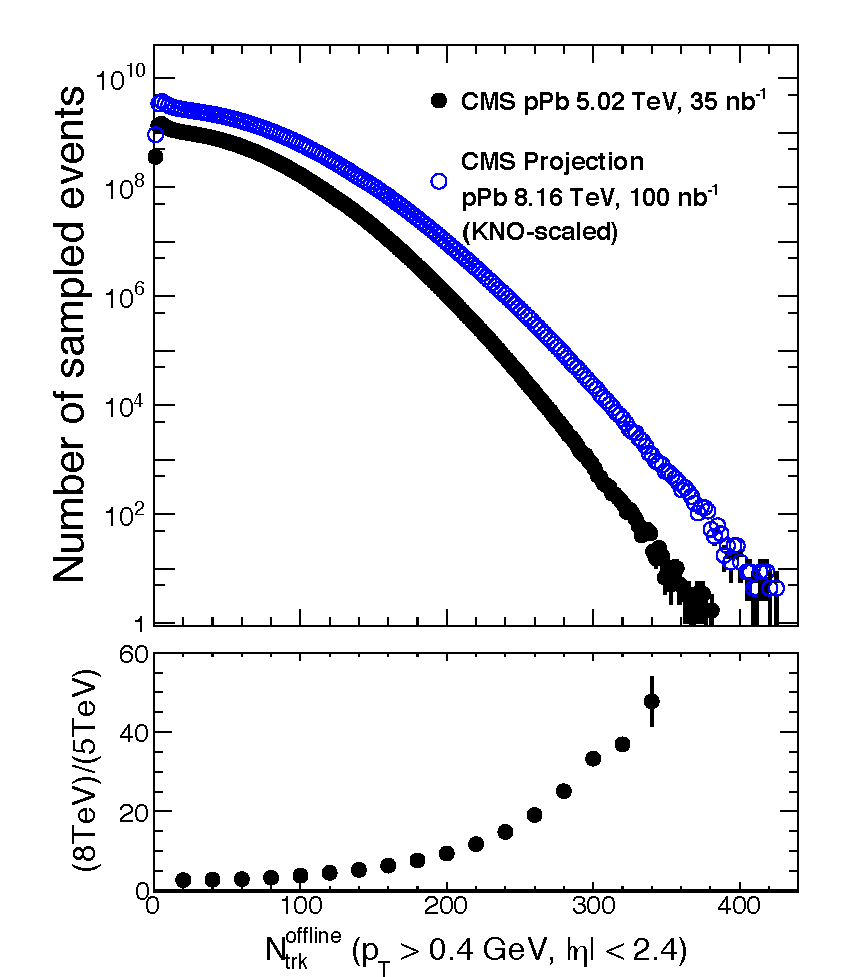
\includegraphics[width=0.6\textwidth]{figures/Ntrk.pdf}
    \caption{ Projected charged particle multiplicity distribution for pPb 
    collisions at \rootsNN\ = 8.16 TeV with L$_{\rm int}$ = 100 nb$^{-1}$
    based on the KNO scaling of measured distribution at \rootsNN\ = 5.02 TeV.
    }
    \label{fig:Ntrk_pPb}
  \end{center}
\end{figure}

Based on an approximate KNO scaling of multiplicity distribution at different collision 
energies, a projection of multiplicity distribution for pPb collisions at \rootsNN\ = 8.16 
TeV is presented in Fig.~\ref{fig:Ntrk_pPb}, corresponding to an integrated luminosity 
of 100 nb$^{-1}$. A ratio of multiplicity distributions at \rootsNN\ = 8.16 TeV 
to \rootsNN\ = 5.02 TeV (L$_{\rm int}$ = 35 nb$^{-1}$) is also shown in the bottom panel of Fig.~\ref{fig:Ntrk_pPb} (Note that the KNO scaling is known to be not exact so the ratio 
is likely to be a little underestimated, especially at large $N_{\rm trk}$ values). 
As one can see, significant enhancement in high-multiplicity event sample is expected 
in 2016 pPb run. The enhancement factor increases as a function of multiplicity owing 
to the increase of collision energy. For instance at $N_{\rm trk}$ value $\approx$ 250, 
20 times more events are expected comparing to 2013 pPb data sample at \rootsNN\ = 5.02 TeV
(a factor of 7 from higher collision energy).

\begin{figure}[t!]
  \begin{center}
    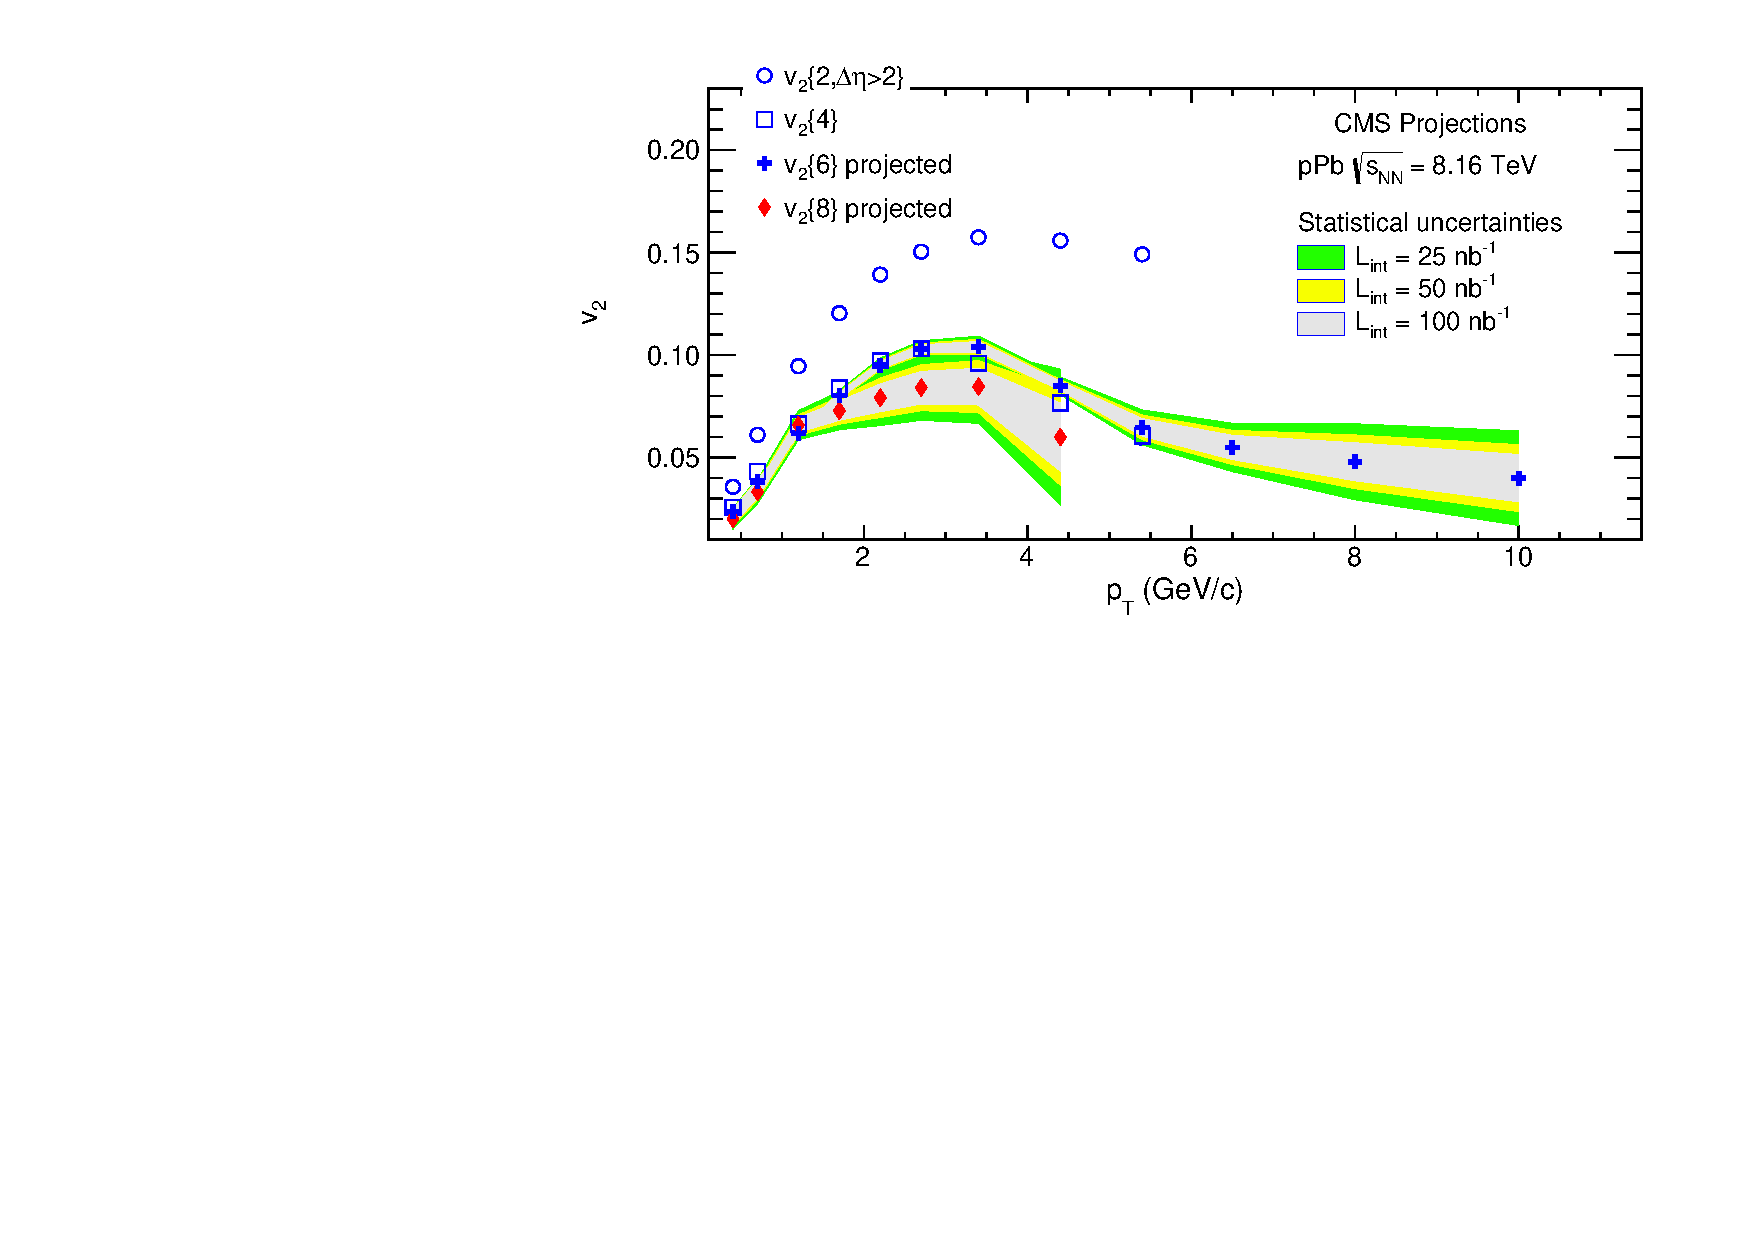
\includegraphics[width=\textwidth]{figures/vnpT_proj_100nb_combineLumi.pdf}
    \caption{ Projected statistical uncertainties of $v_2\{6\}$ and $v_2\{8\}$ as a function of \pt\ 
    for pPb collisions at \rootsNN\ = 8.16 TeV, based on data at \rootsNN\ = 5.02 TeV, with luminosity
    scenarios of L$_{\rm int}$ = 100, 50 and 25 nb$^{-1}$. Data points for $\pt<6$ GeV/c
    are directly taken from 5.02 TeV measurement while $v_{2}\{6\}$ values for $\pt>6$ GeV/c
    are hypothetical, mainly for demonstrating the statistical sensitivity at very high \pt.
    }
    \label{fig:vnpT}
  \end{center}
\end{figure}

Following the observation of collectivity for $\pt$-inclusive 
particles~\cite{Khachatryan:2015waa} (Fig.~\ref{fig:ridge_pPb}, right), 
a natural question to pursue is whether this collectivity extends differentially 
in particle \pt\ to higher \pt\ regime. First attempt has been 
made using run-1 pPb data, where $v_2$ is measured 
by correlating one particle at different \pt\ with multiple low-\pt\ particles 
($0.3<\pt<3$ GeV/c) in high-multiplicity pPb collisions~\cite{CMS-PAS-HIN-15-008}.
Due to statistical limitation, it is not possible to conclude on the relation of $v_{2}$
values extracted from four-, six- and eight-particle correlations as a function of \pt.

Figure~\ref{fig:vnpT} shows the projected statistical precision for $v_{2}\{6\}$
and $v_{2}\{8\}$ as a function of \pt\ that can be achieved in 2016 pPb run at 
\rootsNN\ = 8.16 TeV. Three different integrated luminosity scenarios of L$_{\rm int}$ = 
100, 50 and 25 nb$^{-1}$ are presented. Data points for $\pt<6$ GeV/c are directly 
taken from 5.02 TeV measurement, while $v_{2}\{6\}$ values for $\pt>6$ GeV/c are 
hypothetical, mainly for demonstrating the statistical sensitivity at very high \pt.
With L$_{\rm int}$ = 100 nb$^{-1}$, the collective nature of particle production 
is expected to be well constrained up to \pt\ about 6 GeV/c.
The $v_2$ value from six-particle correlations can be even explored to \pt\ around 10 GeV/c, 
a regime dominated by hard QCD processes. Observation of a finite $v_2$ value at very 
high \pt, especially via multiparticle correlations, would be indicative 
of medium interactions with hard partons in pPb collisions. A reduced data sample
of, e.g., L$_{\rm int}$ = 50 or 25 nb$^{-1}$ would significantly compromise 
the goal of exploring this exciting physics, as illustrated in the figure.

\begin{figure}[t!]
  \begin{center}
    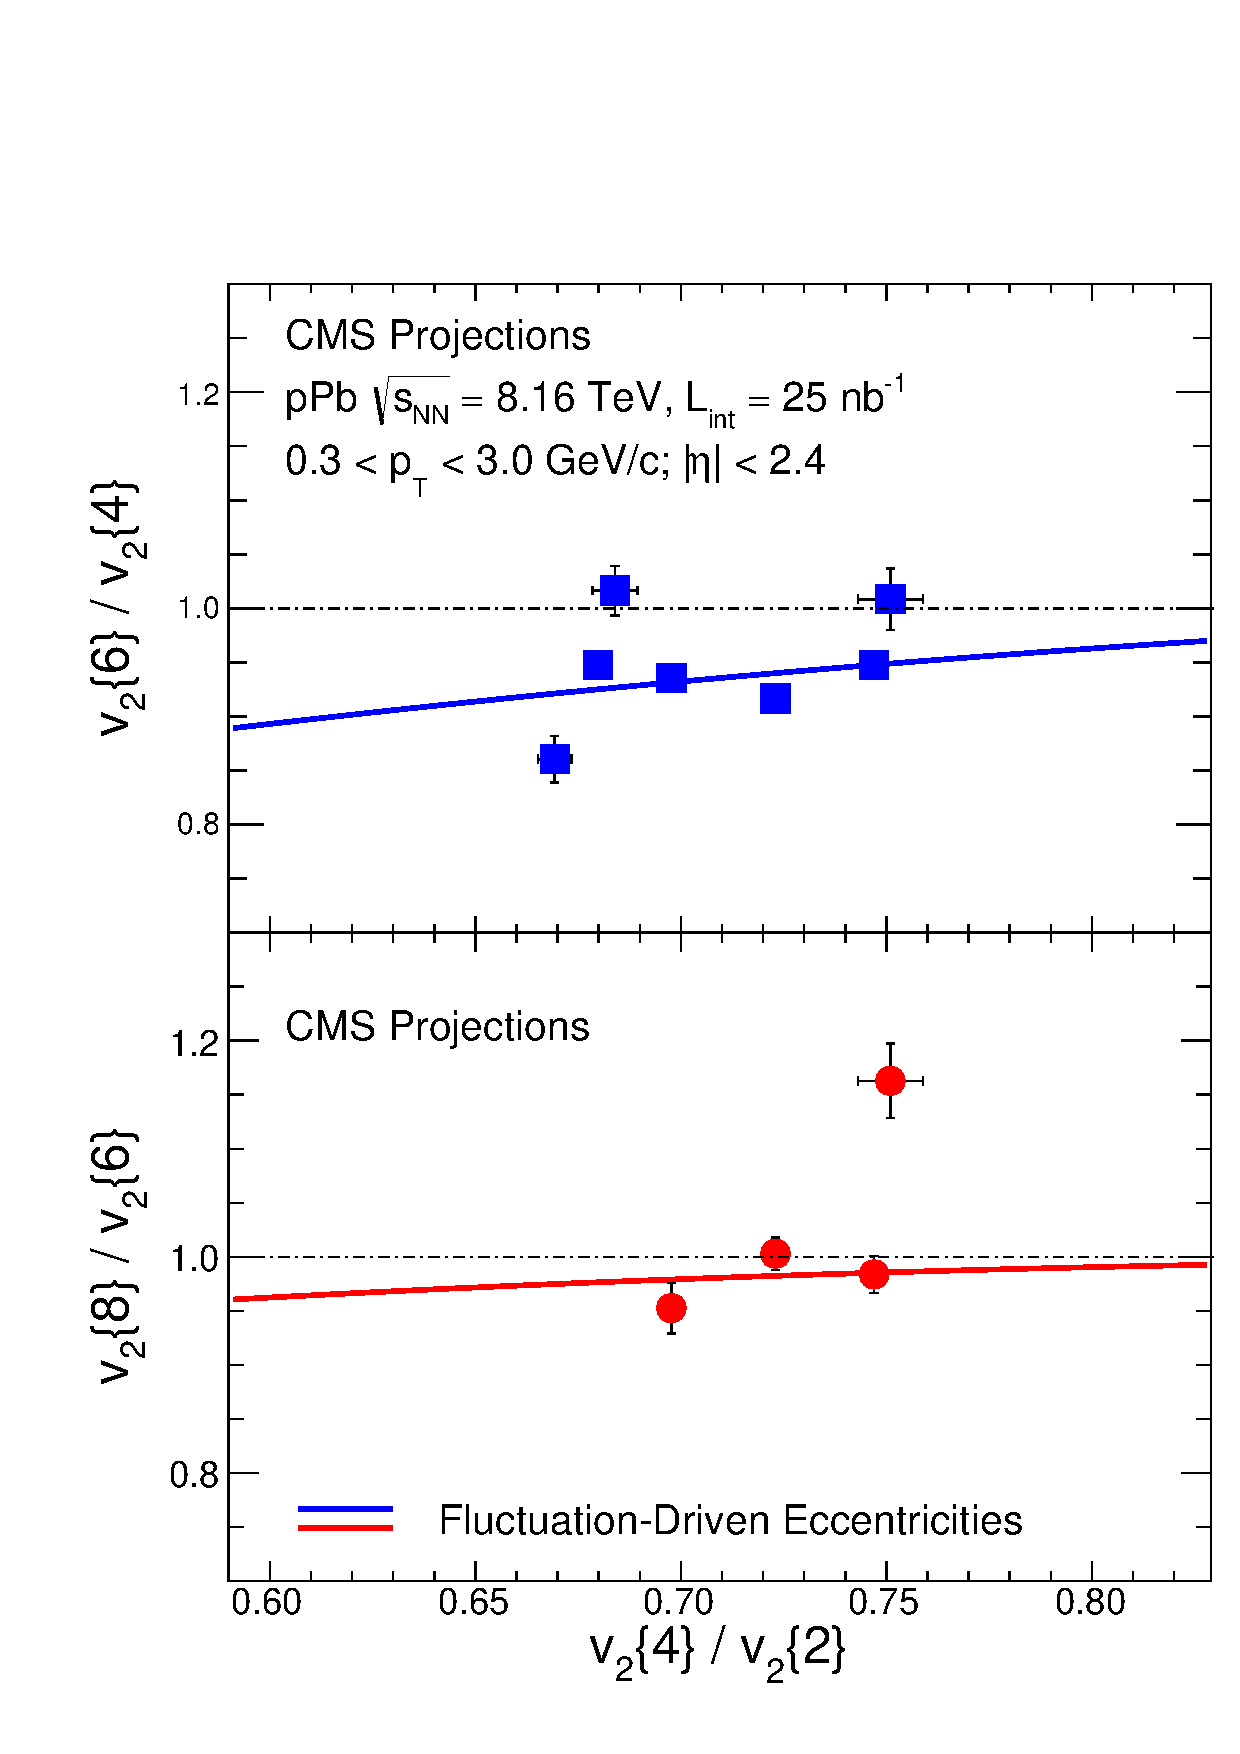
\includegraphics[width=0.5\textwidth]{figures/vnRatios_proj_100nb.pdf}
    \caption{ Projected statistical uncertainties of $v_2\{4\}/v_2\{2\}$, $v_2\{6\}/v_2\{4\}$ and $v_2\{8\}/v_2\{6\}$ ratios
    for pPb collisions at \rootsNN\ = 8.16 TeV with L$_{\rm int}$ = 100 nb$^{-1}$, based on data at \rootsNN\ = 5.02 TeV.
    }
    \label{fig:vnNtrk}
  \end{center}
\end{figure}

Once the collective nature of particle production is established, 
the next question to address is what the underlying mechanism is in 
driving the collectivity. Specifically, the goal of CMS is to 
disentangle different proposed theoretical scenarios such as hydrodynamic models and
gluon saturation models via high precision measurements. 

Hydrodynamic model predicts that $v_2$ is proportional to the 
eccentricity, $\epsilon_{2}$, of the initial colliding system.
Based on initial-state eccentricity fluctuations, a quantitative
relationship among $v_2\{2\}$, $v_2\{4\}$, $v_2\{6\}$ and $v_2\{8\}$ 
has been predicted, denoted as solid curves in Fig.~\ref{fig:vnNtrk}~\cite{Yan:2013laa}. 
While the values of $v_2\{4\}$, $v_2\{6\}$ and $v_2\{8\}$
are expected to be very similar, a few \% deviation is expected in the context of
hydrodynamic scenario. Such a small deviation has been explored in 2013 
pPb run~\cite{Khachatryan:2015waa}. An indication of data being consistent 
with hydrodynamic prediction is seen but it remains inconclusive due to 
statistical limitation. In Fig.~\ref{fig:vnNtrk}, based on the 2013 pPb data, the projected statistical
uncertainties of $v_2\{6\}/v_2\{4\}$ and $v_2\{8\}/v_2\{6\}$ versus
$v_2\{4\}/v_2\{2\}$ ratios in high-multiplicity pPb collisions for 2016 run
are shown, assuming an integrated luminosity of 100 nb$^{-1}$.
Owing to the higher collision energy and luminosity, statistical precision 
of these ratio measurements are expected to reach a level of 2--3\%.
A more solid conclusion can be achieved in comparing the data with model predictions.